\section{矢量数据库的应用场景}

矢量数据库的最典型应用场景,就是与深度学习模型相结合,基于深度学习模型将数据变换为矢量后,存储在数据库中,之后利用数据库系统的内置函数进行匹配。

\begin{figure}[H]
    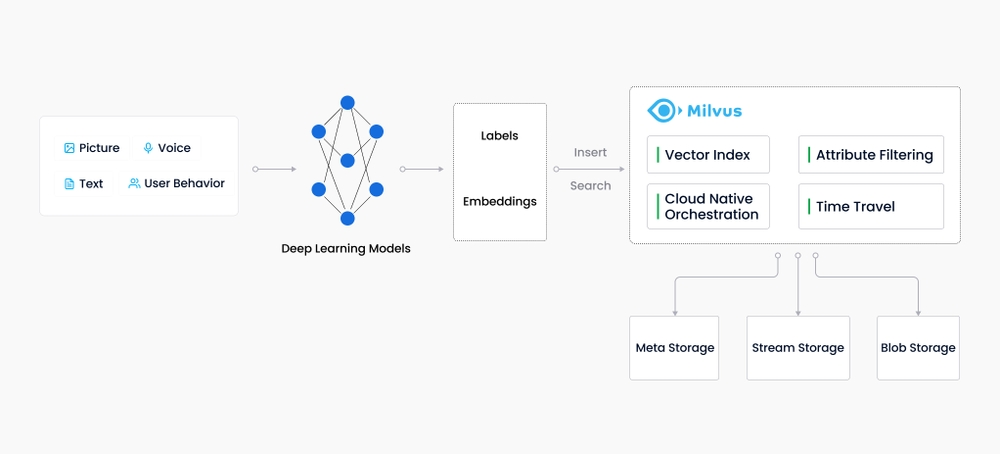
\includegraphics[width=\textwidth]{examples/milvus.jpg}
    \centering
    \caption{矢量数据库Milvus的应用}
    \label{fig:milvus}
\end{figure}

如图\ref{fig:milvus}所示,图像、语音、文本甚至用户行为等信息都可以通过深度学习模型编码成矢量,并与标签(即元数据)附加在一起送入矢量数据库Milvus中进行存储。之后,就可以调用Milvus的一系列方法进行任务。

这里将介绍矢量数据库的2种典型应用场景,图像检索和搜索引擎。

\subsection{图像检索}

图像检索指的是通过指定的一些信息,从大量图像种找到最适合的一系列图像。指定的信息可以是文本、图像或其他信息,这里介绍一个以图搜图的案例。

使用现有模型VGG\cite{simonyan2014very}/ResNet\cite{he2016deep}等深度学习模型,可以将图像编码成矢量的形式。图\ref{fig:vgg}展示了VGG的模型结构,输入尺寸为$224\times 224$的图像,VGG通过若干层卷积、池化和线性变换操作将其映射到一个长度为4096的矢量。

\begin{figure}[H]
    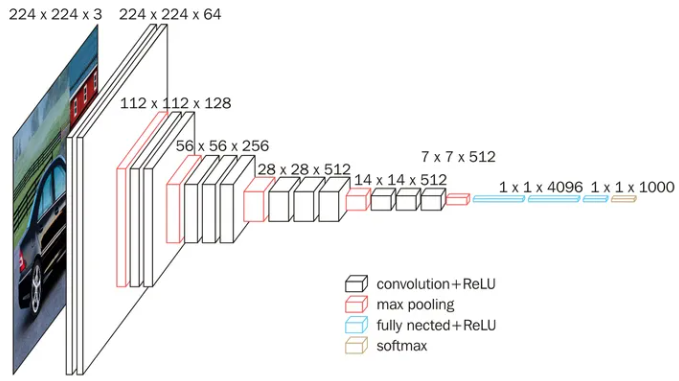
\includegraphics[width=0.6\textwidth]{examples/vgg.png}
    \centering
    \caption{VGG模型}
    \label{fig:vgg}
\end{figure}

我们可以将大量图像通过VGG转换为矢量之后存入矢量数据库中,之后对于一张新的图像,只需要也将其转换为矢量,就可以利用矢量数据库找到其中最相近的图像。图\ref{fig:pic2pic}展示了这一详细流程。

\begin{figure}[H]
    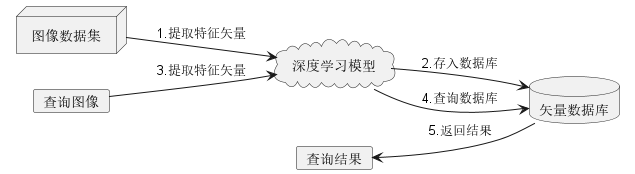
\includegraphics[width=\textwidth]{examples/pic2pic.png}
    \centering
    \caption{基于矢量数据库的图像检索工作流程}
    \label{fig:pic2pic}
\end{figure}

基于Milvus,可以很容易实现上述功能。Milvus提供了丰富的接口,供用户上传和查询矢量,下面是一个简单的以图搜图案例展示。如图\ref{fig:pic2pic_demo}所示,上传一张猫的图像,该系统可以帮助我们找到相似的猫的图像,并返回相似度信息。

\begin{figure}[H]
    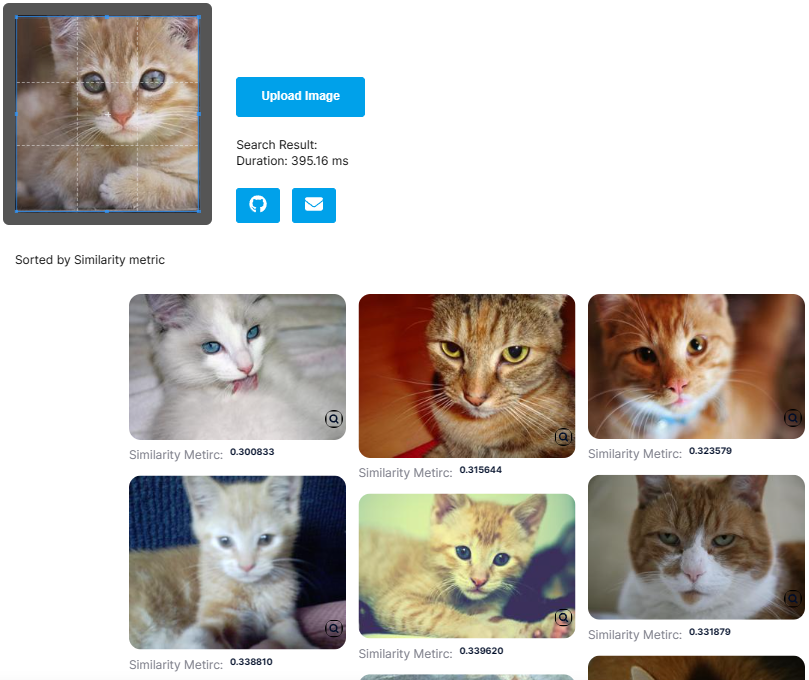
\includegraphics[width=0.7\textwidth]{examples/pic2pic demo.png}
    \centering
    \caption{以图搜图案例}
    \label{fig:pic2pic_demo}
\end{figure}

\subsection{搜索引擎}

同样的,矢量数据库可以用作搜索引擎,只需将大量文本内容编码为矢量后存入数据库,再将搜索内容同样编码为矢量之后,与库中进行匹配,找到最相似的矢量对应的文本内容即可。

为了实现文本内容的编码,这里介绍一个经典的自然语言处理模型BERT\cite{devlin2018bert}。如图\ref{fig:bert}所示,BERT模型能够将输入的文本序列编码为一组深度的token序列。

\begin{figure}[H]
    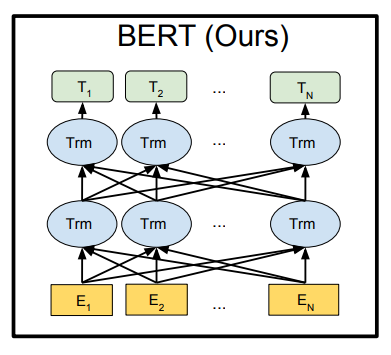
\includegraphics[width=0.4\textwidth]{examples/bert.png}
    \centering
    \caption{BERT}
    \label{fig:bert}
\end{figure}

于是,基于矢量数据库的搜索引擎可以以如下形式构建。如图\ref{fig:search_engine}所示,大量文档的标题通过BERT模型编码为矢量后,存入Milvus矢量数据库中(蓝色线条)。之后待搜索文本同样通过BERT编码为矢量后,就可以在Milvus中寻找匹配矢量(橙色线条)。需要注意的是,这里还引入了关系型数据库PostgreSQL来保存文档本身的内容,Milvus会返回文档号,之后就可以通过文档号在关系型数据库中获取文档本身的内容。

\begin{figure}[H]
    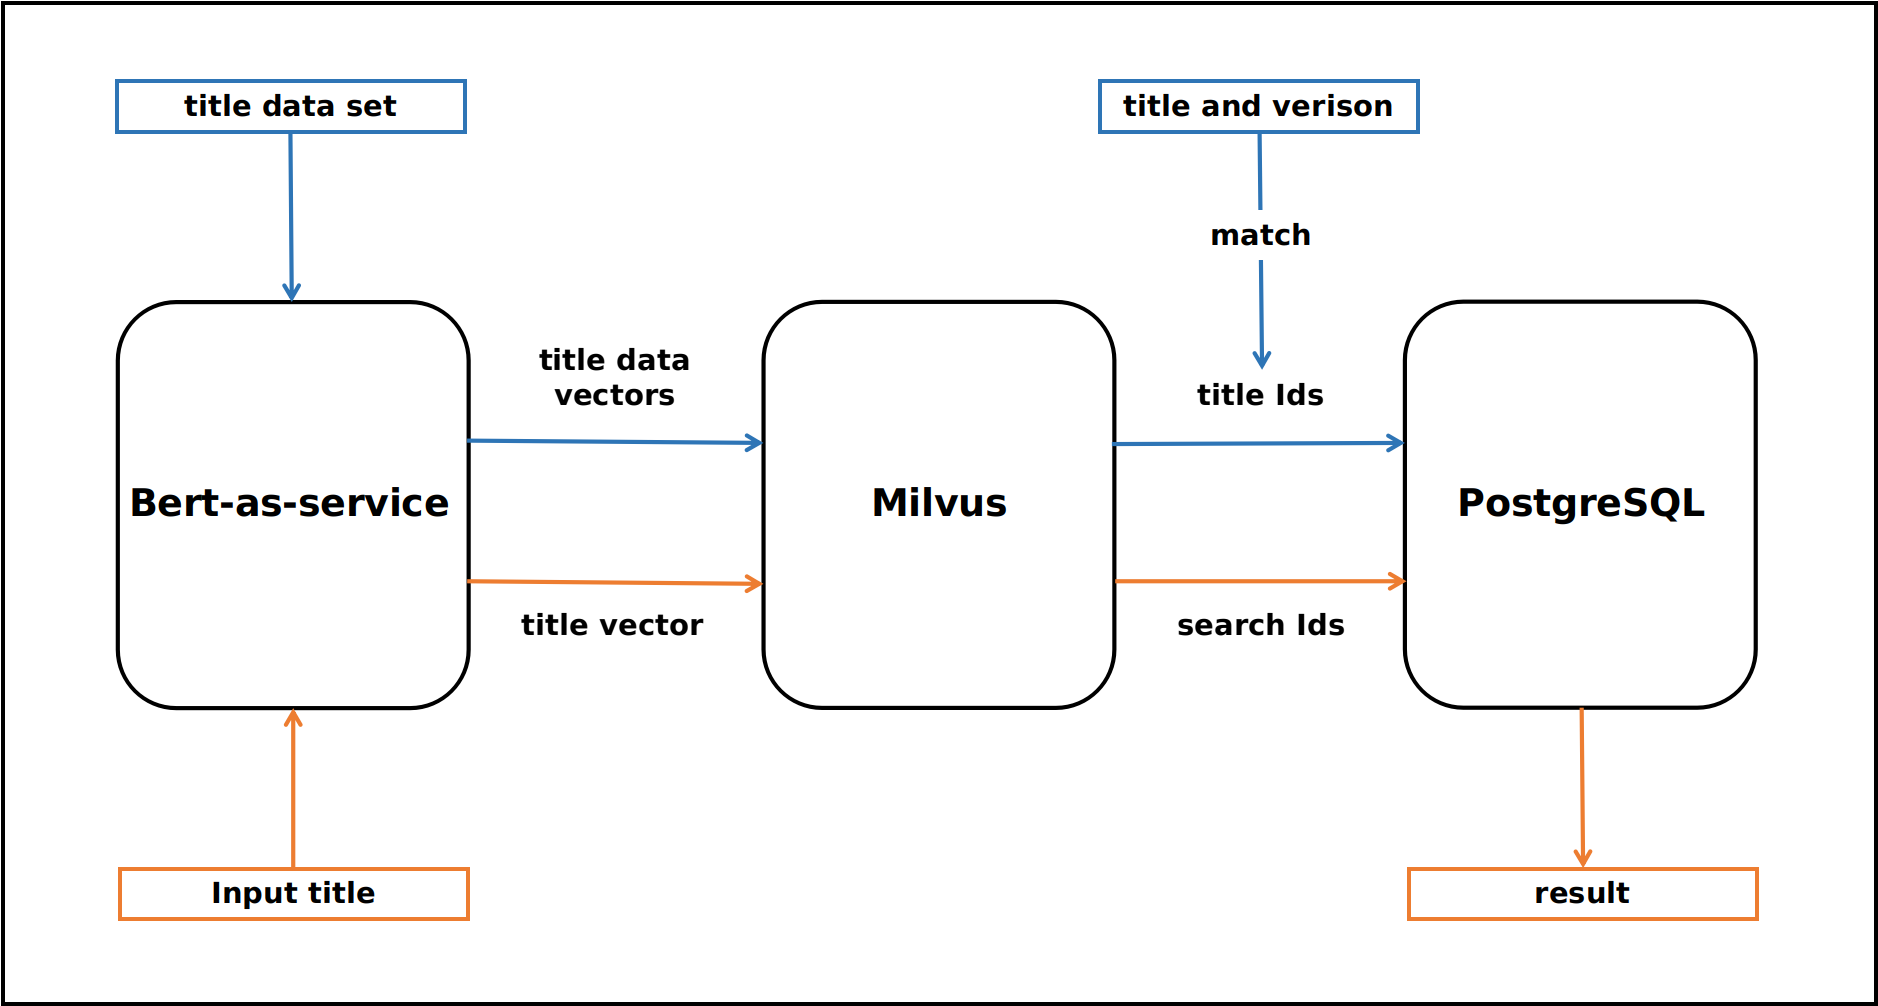
\includegraphics[width=0.7\textwidth]{examples/search engine.png}
    \centering
    \caption{基于矢量数据库的搜索引擎工作流程}
    \label{fig:search_engine}
\end{figure}

这里同样展示了一个搜索引擎的简单案例,如图\ref{fig:search_engine_demo}所示,输入文本内,该案例可以返回相似的一些文档内容。

\begin{figure}[H]
    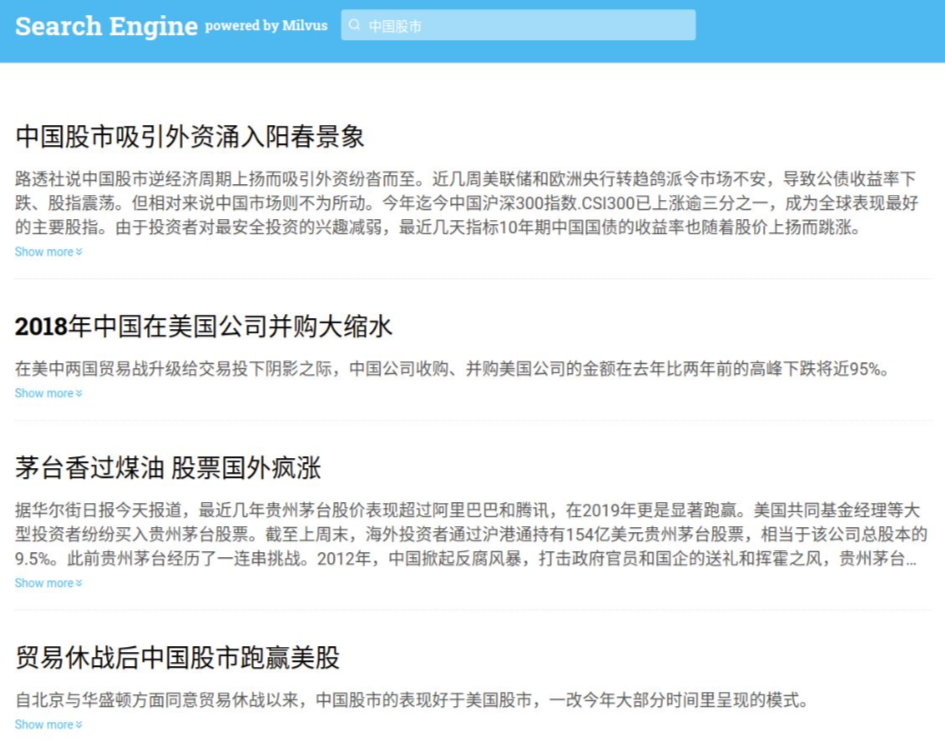
\includegraphics[width=0.7\textwidth]{examples/search engine demo.png}
    \centering
    \caption{搜索引擎案例}
    \label{fig:search_engine_demo}
\end{figure}